\documentclass[10pt,twoside]{report}
\usepackage{charter,titlesec,fancyhdr,wrapfig,framed}
\usepackage[pdftex]{graphicx}
\usepackage{colortbl}
\definecolor{white}{gray}{1.0}
\definecolor{gray-5}{gray}{0.95}
\definecolor{gray-10}{gray}{0.9}
\definecolor{gray-20}{gray}{0.8}
\definecolor{gray-30}{gray}{0.7}
\definecolor{gray-40}{gray}{0.6}
\definecolor{fadered}{rgb}{0.8824, 0.9529, 0.8745}
\usepackage{subfigure}
\usepackage[papersize={6.8in,8.8in},left=2cm,right=2cm,top=3cm,bottom=2cm]{geometry}
\usepackage{setspace}
\usepackage[charter]{mathdesign}
\usepackage[small]{caption}
\usepackage[scaled]{beramono}
\usepackage{abstract}
\usepackage{nextpage}
\usepackage{picins}

\usepackage{listings} 
%\lstset{numbers=left, numberstyle=\scriptsize\ttfamily, numbersep=10pt, captionpos=b} 
\lstset{backgroundcolor=\color{white}}
\lstset{basicstyle=\small\ttfamily}
\lstset{framesep=4pt}
\lstset{language={}}
\newcommand{\inlineCode}{\lstinline[basicstyle=\normalsize\ttfamily]}

\usepackage[colorlinks=true,linkcolor=black,citecolor=black,urlcolor=black,filecolor=black,bookmarks=true]{hyperref}
\hypersetup{
pdfauthor = {Michael Specht},
pdftitle = {Proteomatic},
pdfsubject = {},
pdfkeywords = {},
pdfcreator = {LaTeX},
pdfproducer = {pdflatex}}

%\usepackage{eso-pic}
\usepackage{color}
\usepackage{type1cm}
\makeatletter
  \AddToShipoutPicture{%
    \setlength{\@tempdimb}{.5\paperwidth}%
    \setlength{\@tempdimc}{.5\paperheight}%
    \setlength{\unitlength}{1pt}%
    \put(\strip@pt\@tempdimb,\strip@pt\@tempdimc){%
      \makebox(0,0){\rotatebox{12}{\textcolor[gray]{0.86}{
        \fontsize{2.4cm}{2.4cm}\selectfont{preliminary \linebreak copy}}}}
    }
}
\makeatother


\include{chapterleft}
\fboxsep0pt
\fboxrule0.05pt

\newcommand{\image}[5]{
  \begin{figure}[htbp]
    \centering
    \includegraphics[width=#3\textwidth]{#2}
    \caption[#5]{#4}
    \label{fig:#1}
  \end{figure}
}

\newcommand{\imageFrame}[5]{
  \begin{figure}[htbp]
    \centering
    \fbox{
      \includegraphics[width=#3\textwidth]{#2}
    }
    \caption[#5]{#4}
    \label{fig:#1}
  \end{figure}
}


\setlength{\parskip}{2mm}
\setlength{\parindent}{0mm}
\renewcommand{\baselinestretch}{1.2} 
\renewcommand{\arraystretch}{1.2} 

\renewcommand{\headrulewidth}{0.25pt}

\pagestyle{fancy}

\renewcommand{\chaptermark}[1]{\markboth{#1}{}}
\renewcommand{\sectionmark}[1]{\markright{#1}}

%\setlength{\marginparwidth}{1.5cm}
%\newcommand{\note}[1]{\marginpar{\color{gray-40}\footnotesize \flushleft #1}}
\newcommand{\note}[1]{}

\newcommand{\imageCourtesy}[2]{Image courtesy of #1 \cite{#2}.}

\fancyhf{}
\fancyhead[EL,OR]{\thepage}
\fancyhead[ER]{\leftmark}
\fancyhead[OL]{\rightmark}
\fancypagestyle{plain} {
  \fancyhf{}
  \renewcommand{\headrulewidth}{0pt}
}

\lstnewenvironment{todo}{\lstset{numbers=none,frame=none,backgroundcolor=\color{fadered}}}{}

\begin{document}

\pagestyle{empty}
\begin{titlepage}
\begin{center}
%\normalfont\noindent\bf\Huge{Interactive Glyph-based 3D Visualization \linebreak of
%Dynamic PET Datasets}
\vspace*{2cm}
\normalfont\noindent\bf\Huge{Proteomatic}

\vfill

\normalfont\noindent\large{a documentation written by}

\vspace*{-0.2cm}

\normalfont\noindent\large{\em Michael Specht}
\end{center}
\end{titlepage}

\cleartoevenpage
\setcounter{page}{2}
\setcounter{tocdepth}{1}
\setcounter{secnumdepth}{2}
\tableofcontents
\newpage

\thispagestyle{empty}

%\cleardoublepage
\pagestyle{fancy}

\fancypagestyle{plain} {
  \renewcommand{\headrulewidth}{0.25pt}
  \fancyhf{}
  \fancyhead[EL,OR]{\thepage}
}
\cleartoevenpage


\chapter{Introduction}

\clearpage


\section{Proteomatic}

Proteomatic is the Proteomics researcher's swiss army knife.  It provides a user interface for both open source and commercial Proteomics software.  Tools can be chained together in a pipeline, and it's availble for Linux, Mac and Windows.

	\parpic[l]{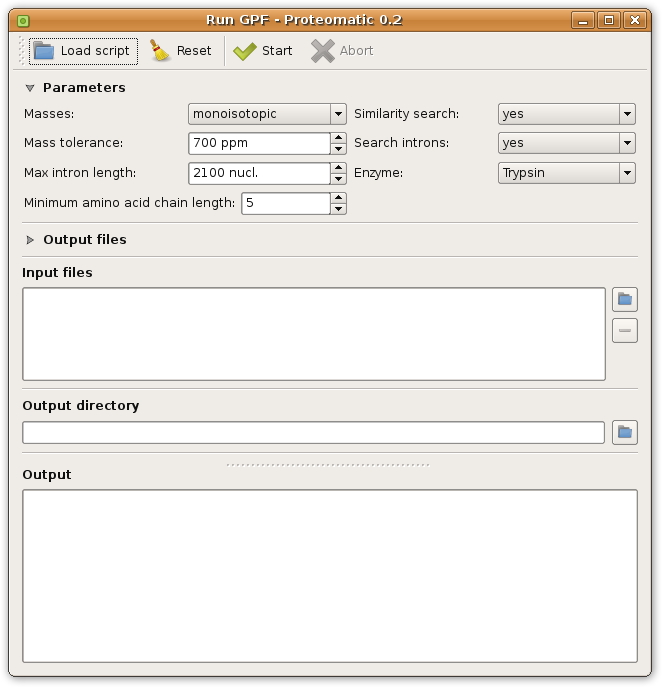
\includegraphics[width=0.5\textwidth]{proteomatic.jpg}} 

This is just some text. It flows! This is just some text. It flows! This is just some text. It flows! This is just some text. It flows! This is just some text. It flows! This is just some text. It flows! This is just some text. It flows! This is just some text. It flows! This is just some text. It flows! This is just some text. It flows! This is just some text. It flows! This is just some text. It flows! This is just some text. It flows! This is just some text. It flows! This is just some text. It flows! This is just some text. It flows! This is just some text. It flows! This is just some text. It flows! This is just some text. It flows! This is just some text. It flows! This is just some text. It flows! This is just some text. It flows! This is just some text. It flows! This is just some text. It flows! This is just some text. It flows! This is just some text. It flows! This is just some text. It flows! This is just some text. It flows! This is just some text. It flows! This is just some text. It flows! This is just some text. It flows! This is just some text. It flows! This is just some text. It flows! This is just some text. It flows! This is just some text. It flows! This is just some text. It flows! This is just some text. It flows! This is just some text. It flows! This is just some text. It flows! This is just some text. It flows! This is just some text. It flows! This is just some text. It flows! This is just some text. It flows! This is just some text. It flows! This is just some text. It flows! This is just some text. It flows! This is just some text. It flows! This is just some text. It flows! This is just some text. It flows! This is just some text. It flows! This is just some text. It flows! This is just some text. It flows! This is just some text. It flows! This is just some text. It flows! This is just some text. It flows! This is just some text. It flows!
\cleartoevenpage


\chapter{Development}

\clearpage


\section{Adding scripts}

A Proteomatic script consists of two parts:

\begin{enumerate}
\item {\bf The script description.} 

This YAML file contains the title, description and options of  the script.


\item {\bf The script.} 

This file contains the Ruby script itself.


\end{enumerate}



\subsection{The script description file}



The filename of the script description file is \lstinline[breaklines=true]�scripts/include/properties/example.yaml�.



\subsection{The script file}



The filename of the script file is \lstinline[breaklines=true]�scripts/example.rb�. The skeleton of a Proteomatic script  looks like this:


\begin{lstlisting}

 require 'include/proteomatic'

 class Example < ProteomaticScript
     def run()
     end
 end

 lk_Object = Example.new

\end{lstlisting}


The \lstinline[breaklines=true]�require 'include/proteomatic'� must be the first line. Then, a subclass of  \lstinline[breaklines=true]�ProteomaticScript� is defined which is instanciated as \lstinline[breaklines=true]�lk_Object� after that. Within the \lstinline[breaklines=true]�run� method, several member variables can be accessed:

\begin{enumerate}
\item {\bf Input files.}  

 For processor scripts, all input files are stored in the \lstinline[breaklines=true]�@input� hash, which has an array of absolute input file paths for each input group key. 


\item {\bf Output files.}  

 For processor scripts, ... yar de yar yar. 


\end{enumerate}

And there's even more!


\section{Adding external tools}

Tools can be added, too! ``{\bf Wow}'', you say.
\end{document}
